\chapter{Introduction}

Word Sense Disambiguation(WSD) is a notoriously difficult problem in understanding text. Ambiguity is very common in text but humans are so competent at figuring out the word sense from context that most of the time they do not notice the ambiguity in the meaning of the word. Accurate sense disambiguation would benefit a number of Natural Language applications; however it is generally acknowledged by WSD researchers that current accuracy levels need to be improved before WSD technology can be usefully integrated into applications \citep{ide2006making}.

There are two major problems faced by the researchers in this area. One major problem is the dearth of sufficient training data for supervised systems. With handful of sense-tagged texts currently available, existing WSD systems don't have examples for all the senses of a word most of the times. The other major problem that automatic disambiguation systems face is the fine-grainedness of the sense-distinctions in the sense inventory, WordNet in our case. 

WordNet \citep{miller1995wordnet} \citep{fellbaum1998wordnet} is well known to the Natural Language Processing community as a valuable resource and is one of the most widely used lexical resource. WordNet being a fine grained sense inventory makes it hard even for humans to reliably and consistently distinguish among word senses. In this thesis we would be addressing the latter problem and produce graded word sense relationships which can be used to derive coarse sense clusters with required granularity.

%more and more applications requiring machine readable dictionaries or world knowledge encoded as a semantic network use WordNet as the underlying sense inventory.

\section{Motivation}

Lets observe the inter-annotator agreement estimates of the data preparation for the Senseval/SemEval tasks on WSD(All Words or Lexical Sample) in table \ref{tab:itaWSD}.

\begin{center}
\begin{longtable}{| c | c | c | c | c | c |}      
    \hline
Workshop and Task & WordNet Version & Verb & Noun & Adjectives & Overall \\\hline 
Senseval-2 AW\footnote{Only approximate information on ITA is available} & \multirow{2}{*}{1.7} & \multirow{2}{*}{70-80} & \multirow{2}{*}{NA} & \multirow{2}{*}{NA} & \multirow{2}{*}{NA} \\ 
\citep{Senseval2AllWordsTask} & & & & & \\ \hline

Senseval-2 LS & \multirow{2}{*}{1.7} & \multirow{2}{*}{NA} & \multirow{2}{*}{86.3} & \multirow{2}{*}{83.4} & \multirow{2}{*}{NA} \\ 
\citep{Senseval2LexicalSampleTask} & & & & & \\ \hline

Senseval-3 AW  & \multirow{2}{*}{1.7.1} & \multirow{2}{*}{67.8} & \multirow{2}{*}{74.9} & \multirow{2}{*}{78.5} & \multirow{2}{*}{72.5}\\ 
\citep{Senseval3AllWordsTask} & & & & & \\ \hline

Senseval-3 LS & \multirow{2}{*}{1.7.1} & \multirow{2}{*}{NA} & \multirow{2}{*}{NA} & \multirow{2}{*}{NA} & \multirow{2}{*}{67.3}\\ 
\citep{Senseval3LexicalSample} & & & & & \\ \hline

Semeval 2007 AW & \multirow{2}{*}{2.1} & \multirow{2}{*}{72} & \multirow{2}{*}{86} & \multirow{2}{*}{NA} & \multirow{2}{*}{NA} \\ 
\citep{Semeval2007WSD} & & & & & \\ \hline
\caption{Inter-annotator agreement for Various Data Preparations} 
\label{tab:itaWSD}
\end{longtable}
\end{center}

As the inter-annotator agreement is often considered an upper bound for WSD systems, it is desirable to have a high ITA. \citep{Navigli06meaningfulclustering} believes that a credible upper bound for unrestricted fine-grained WSD is around 70\%, a figure that state-of-the-art automatic systems find difficult to outperform. Therefore it seems that the major bottleneck in effective WSD is the fine grained nature of the WordNet sense inventory, rather than the performance of the best disambiguation systems.

The above points are substantiated by the ITA achieved in preparation of gold standard datasets and performance of the systems in SemEval-2007 Task on Coarse grained WSD \citep{navigli-litkowski:SemEval-2007}. The ITA values on train and test datasets were 86.44\% and 93.80\%. These figures, compared to those in the table \ref{tab:itaWSD}, show that the performance of the WSD systems can be improved by changing the granularity of the adopted sense inventory.

Some of the best systems of the SemEval-2007 Coarse Grained WSD task achieved performances in early 80s in all words task and in high 80s in lexical sample task as compared to previous Senseval evaluation exercises, where state-of-the-art systems achieved performance far below 70\%. This encourages us to study in depth the ideas for good sense clustering algorithms and use them to improve the WSD systems so that they can be used in practical scenarios.

\begin{comment}
To understand the granularity of WordNet, lets take an example.
\begin{example}
Consider the senses of the word \textit{evidence} as a \textit{noun} from WordNet version 3.1\footnote{Online WordNet Search : \url{http://wordnetweb.princeton.edu/perl/webwn}} in the table \ref{tab:evidenceExample}.
For most of the applications the sense distinctions are too-fine and are not required. 
One might say that they are all clearly related. \cite{mccarthy2006relating}
\begin{table}[h]
\centering
\begin{tabular}{ | l | p{12cm} |} 
\hline
WordNet Sense & Gloss \\ \hline
evidence\#n\#1 & evidence, grounds (your basis for belief or disbelief; knowledge on which to base belief)  ``the evidence that smoking causes lung cancer is very compelling`` \\ \hline
evidence\#n\#2 & evidence (an indication that makes something evident) ''his trembling was evidence of his fear'' \\ \hline
evidence\#n\#3 & evidence ((law) all the means by which any alleged matter of fact whose truth is investigated at judicial trial is established or disproved) \\ \hline    
\end{tabular}
\caption{Senses of the word \textit{evidence}} 
\label{tab:evidenceExample}
\end{table}
\end{example}
\end{comment}

\section{WordNet}
WordNet \citep{miller1995wordnet} \citep{fellbaum1998wordnet} is a computational lexicon of English based on psycholinguistic principles, created and maintained at Princeton University\footnote{\url{http://wordnet.princeton.edu}}. Nouns, verbs, adjectives and adverbs are grouped into sets of cognitive synonyms (\textit{synsets}), each expressing a distinct concept. These synsets are then interlinked by means of conceptual-semantic and lexical relations. Additionally, a synset contains a brief definition (“gloss”) and, in most cases, one or more short sentences illustrating the use of the synset members. Word forms with several distinct meanings are represented in as many distinct synsets. Thus, each form-meaning pair in WordNet is unique. We are using WordNet 3.0, which contains 155,287 words organized in 117,659 synsets. \footnote{\url{http://wordnet.princeton.edu/man/wnstats.7WN.html}} 

\noindent
WordNet relations can be summarised as follows :
\begin{itemize}
\item \textit{Lexical Relations} : Lexical relations connect word senses included in the respective synsets
  \begin{itemize}
  \item \textit{Antonymy} : X is an antonym of Y if it expresses the opposite concept (e.g. \textit{good\#a\#1}\footnote{The format we use to express a word sense is \textit{lemma\#POS\#senseNumber}} is the antonym of \textit{bad\#a\#1})
  \item \textit{Pertainymy} : X is an an adjective which can be defined as ``of or pertaining to'' a noun (e.g. \textit{dental\#a\#1} pertains to \textit{tooth\#n\#1})
  \item \textit{Nominalization} : a noun nominalizes a verb Y (e.g. \textit{service\#n\#2} nominalizes the verb \textit{serve\#v\#4})
  \end{itemize}
\item \textit{Semantic Relations} : Semantic Relations apply to synsets in their entirety
  \begin{itemize}
  \item \textit{Hypernymy-Hyponymy-Troponymy} : The most frequently encoded relation among synsets is the super-subordinate relation (also called IS-A relation).
  Y is a hypernym of X if every X is a (kind of) Y. Hypernymy holds between pairs of nominal and verbal synsets. (for e.g. \textit{motor vehicle\#n\#1} is a hypernym of \textit{car\#n\#1}).
  Hyponymy and Troponymy are the inverse relation of hypernymy for nominal and verbal synsets respectively.
  \item \textit{Meronymy-Holonymy} : Y is a meronym of X if Y is a part of X. (e.g. \textit{flesh\#n\#3} is a meronym of \textit{fruit\#n\#1}.
  Holonymy is the inverse relation of meronymy.
  \item \textit{Entailment} : a verb Y is entailed by a verb X if by doing X you must be doing Y (e.g. \textit{snore\#v\#1 entails sleep\#v\#1})
  \item \textit{Similarity} : an adjective X is similar to an adjective Y (e.g. \textit{beautiful\#a\#1} is similar to \textit{pretty\#a\#1})
  \item \textit{Attribute} : A noun X is an attribute for which an adjective Y expresses a value (e.g. \textit{hot\#a\#1} is a value of \textit{temperature\#n\#1})
  \item \textit{See also} : this is a relation of relatedness between adjectives (e.g \textit{beautiful\#a\#1} is related to \textit{attractive\#a\#1} through the \textit{see also} relation)
  \end{itemize}  
\end{itemize}

Figure \ref{fig:excerptFromWordNet} gives an insight into the relationships contained in WordNet \citep{navigli2009WSDSurvey}.
\begin{figure}[h]
\begin{center}
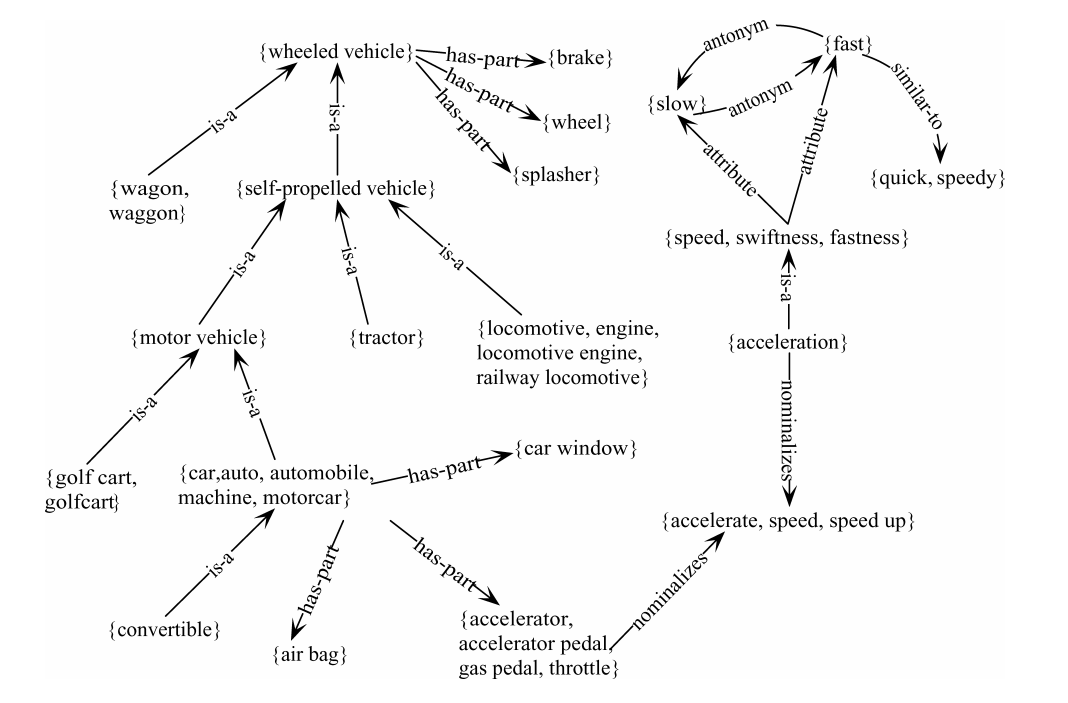
\includegraphics[scale = 0.6]{excerptFromWordNet.png}
\caption{Excerpt From WordNet}
\label{fig:excerptFromWordNet}
\end{center}
\end{figure}

\section{Problem Statement}
\textit{Can we produce and evaluate coarse-grained sense inventories of arbitrary granularity from lexical resources like WordNet and show that they help boost sense disambiguation on standard test sets?}

The problem can be more succinctly defined as follows : Design a system which given a word \textit{w} with its part of speech \textit{p}, lists the senses of the word. The system should be able to control the granularity of sense distinctions.

\subsection{Clustering Synsets Vs Clustering Senses}
For generating a coarse sense inventory, many researchers have focused on clustering WordNet senses into groups i.e. generate coarse senses for each word by merging its senses \citep{agirre2003clustering} \citep{chklovski2003exploiting} \citep{Navigli06meaningfulclustering}. In this approach, we would like to highlight two problems. One problem is that to do this a stopping criterion is required such as the number of clusters required for each word. This has been done with the numbers determined by the gold standard for the purposes of evaluation \citep{agirre2003clustering} but ultimately the right number of classes for each word cannot usually be predetermined even if one knows the application, unless only a sample of words are being handled. Therefore such coarsening systems cannot be used to derive coarse senses for all the words and thus are unable to produce coarse sense inventories. The other problem being the inconsistent sense clusters obtained because of independent generation of coarse senses for 
each word. Even manually done sense clusterings can have this error : consider the sense clusters of the verbs \textit{require} and \textit{need} from Senseval-2 judgements in figure \ref{fig:transitiveError} \citep{snow07mergesense}.

\begin{figure}[h]
\begin{center}
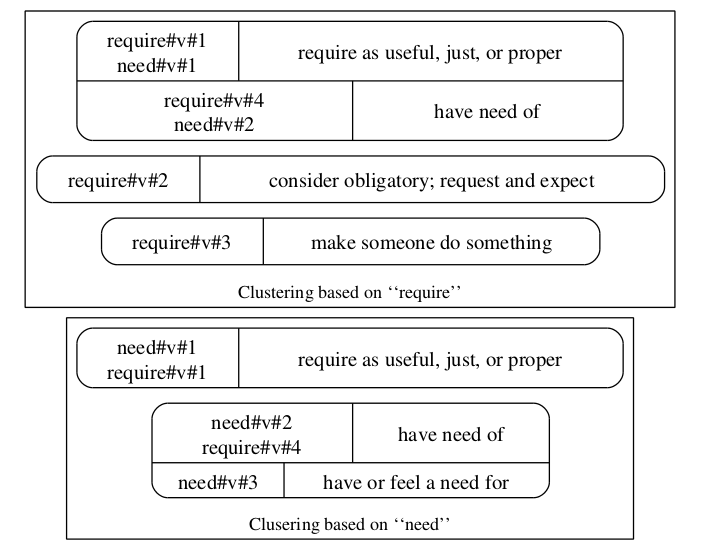
\includegraphics[scale = 0.6]{transitiveError.png}
\caption{Inconsistent sense clusters for the verbs \textit{require} and \textit{need} from Senseval-2 judgements}
\label{fig:transitiveError}
\end{center}
\end{figure}

The two WordNet 2.1 senses \textit{need\#v\#1} and \textit{need\#v\#2} clustered in word specific labelling for \textit{require}, are not clustered according to word-specific labeling for \textit{need}. These transitive closure errors suggest that for deriving consistent coarse senses, we should cluster synsets and not senses.

\begin{comment}
\subsection{Understanding sense clustering}
When we merge two synsets, should we modify the underlying structure of taxonomy as well?
What should be the repercussion of the mergings on the taxonomy?

An important point to note here is that if we merge two synsets and introduce the merged synsets instead of the original synsets in the WordNet taxonomy, either we'll be adding some spurious relations and/or we'll be losing some relationship information.


\subsection{Task Description}
Formally, the task we are attempting has two objectives : 
\begin{enumerate}
\item Given a fine sense inventory and taxonomy like WordNet, we wish to compute a clustering over WordNet synsets at arbitrary granularity, which can serve as a coarse sense inventory. 
\item Assessing the quality of the clustering 
\end{enumerate}

\section{Organization of Thesis}
The rest of this thesis is organized as follows. 
Chapter \ref{chapter:Background}, reviews the algorithms proposed for the task of sense clustering and the evaluation frameworks for the same. 
Chapter \ref{chapter:SupervisedSynsetSimilarity} discusses a supervised attempt to capture WordNet synset similarity using various features derived from WordNet and external corpora. 
Chapter \ref{chapter:Semi-SupervisedSynsetSimilarity}, presents a semi-supervised approach to estimate WordNet synset similarity and describes our approach to produce coarse sense inventory. 
The conclusion is provided in Chapter ????.
\end{comment}